\section{Results} \label{sec:results}
Here the results will be presented. We start looking at how good our linear regression is, by fitting a polynomial to points withdrawn from a known PDF. Thereafter we will see how good the regression is when using real terrain data. To give a intuition on how good the fit is, we will in both cases show 3D plots of the graphs using various methods, and then present the error analysis. 

\subsection{Franke function}
Below one can find the results of the regression on Franke function. All results in this section was obtained from the same data set, with an estimated variance of ...

\subsubsection{Visualization of graphes}
In figure \eqref{fig:data} one can find a 3D visualization of the Franke function, for easier comparison with the fitted graphs presented in figure \eqref{fig:franke_plots}. The data sets were composed drawing random $x$'s and $y$'s in the interval $x,y\in[0,1]$ from a uniform distribution, and the corresponding $z$-values where obtained from the Franke function. Further, we added noise produced by $\mathcal{N}(0, \sigma^2=0.1)$ and compared with the undisturbed data set. For Lasso and Ridge, we used a penalty $\lambda=1e-15$, and for Lasso we also used gradient descent for minimization. On that occasion, the learning rate was set to $\eta=0.001$ with niter$=1000000$ as the number of iterations. 

 
\newgeometry{left=2cm,right=2cm,top=1cm}
\begin{figure} [H]%
    \centering
    \subfloat[OLS without noise]{{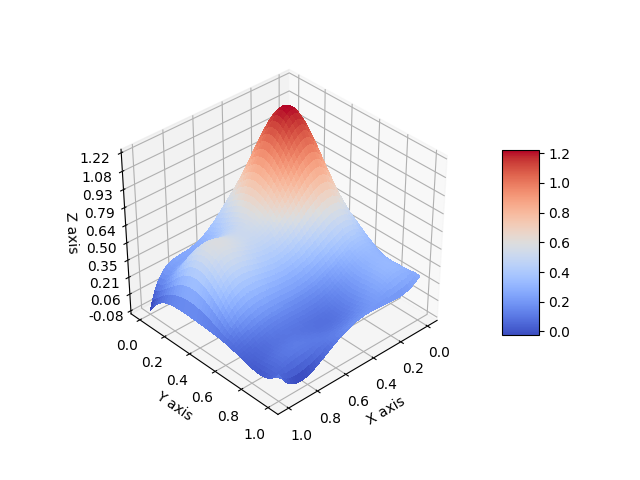
\includegraphics[width=9cm]{../plots/OLS.png} }}%
    \subfloat[OLS with noise]{{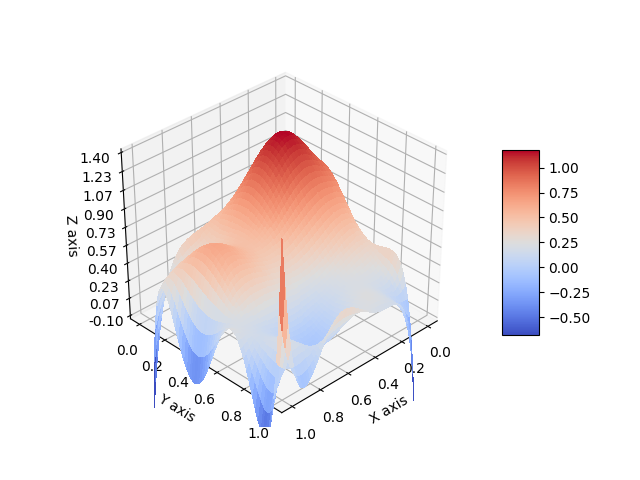
\includegraphics[width=9cm]{../plots/OLS_noise.png} }}\\

    \subfloat[Ridge without noise]{{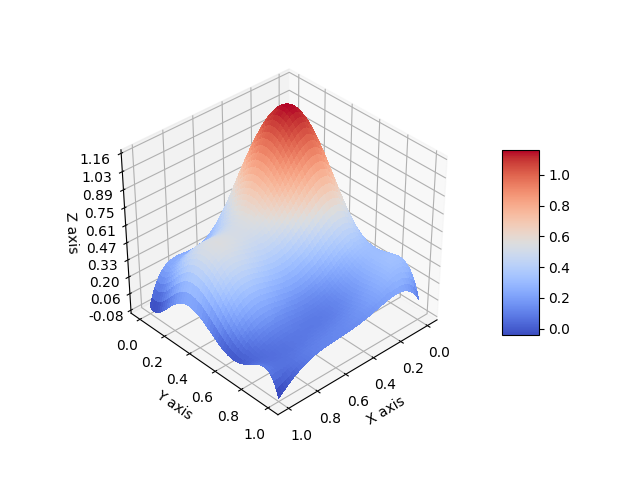
\includegraphics[width=9cm]{../plots/Ridge.png} }}%
    \subfloat[Ridge with noise]{{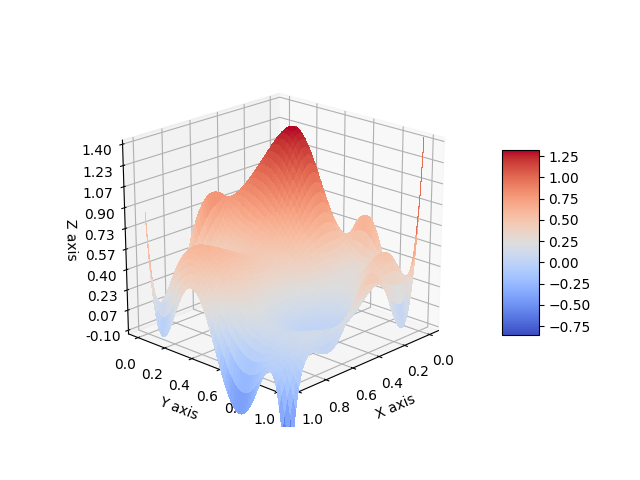
\includegraphics[width=9cm]{../plots/Ridge_noise.png} }}\\
    
    \subfloat[Lasso without noise]{{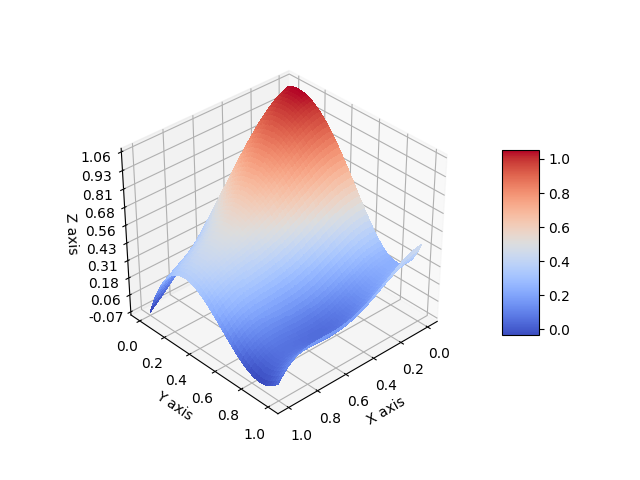
\includegraphics[width=9cm]{../plots/Lasso.png} }}%
    \subfloat[Lasso with noise]{{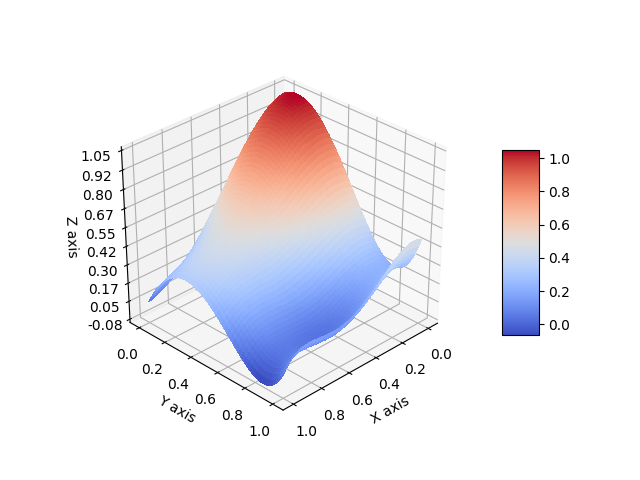
\includegraphics[width=9cm]{../plots/Lasso_noise.png} }}
    \caption{Fitted polynomial by OLS, Ridge and Lasso with and without noise. For Ridge and Lasso, we used a low penalty of $\lambda=1e-15$. Lasso was performed with $\eta=1e-3$ and 1e6 iterations. The noise was sampled from a normal distribution with $\sigma=0.1$.}%
    \label{fig:franke_plots}%
\end{figure}
\restoregeometry


\subsubsection{Error}
To be able to determine which method is best, we need to analyze the error. In table \eqref{tab:franke_error}, the MSE and R$^2$-score are given for OLS, Ridge, Lasso and Ridge with gradient descent. 

\begin{table} [H]
	\caption{Mean Square Error and R$^2$-score presented for OLS, Ridge, Lasso and Ridge + gradient descent.  \vspace{2mm}}
	\begin{tabularx}{\textwidth}{l|XX|XX} \hline\hline
		\label{tab:franke_error}
		& \multicolumn{2}{c}{\textbf{MSE}}&\multicolumn{2}{c}{\textbf{R2}}\\ \hline
		&self&scikit&self&scikit\\ \hline \\
		OLS & 0.07853 & 0.86104 & 0.05386 & 1.7483\\
		Ridge & 0.07852 & 0.86410 & 0.05406 & 1.6904 \\
		Lasso & 0.07704 & 0.86231 & 0.07187 & 1.6492 \\
		RidgeGD & 0.07523 & 0.91850 & 0.09362 & 1.3217 \\ \hline
	\end{tabularx}
\end{table}


\subsubsection{Coefficients $\beta$}
It can also be interesting to see how the coefficients actually differ between the self-built functions and the Scikit Learn function. In figure \eqref{fig:beta_plots}, the beta values are visualized such that large numbers got strong color, negative numbers are blue and positive numbers are red. The methods OLS, Ridge, Lasso and Ridge produced using gradient descent are presented. 

\begin{figure} [H]%
	\centering
	\subfloat[OLS self]{{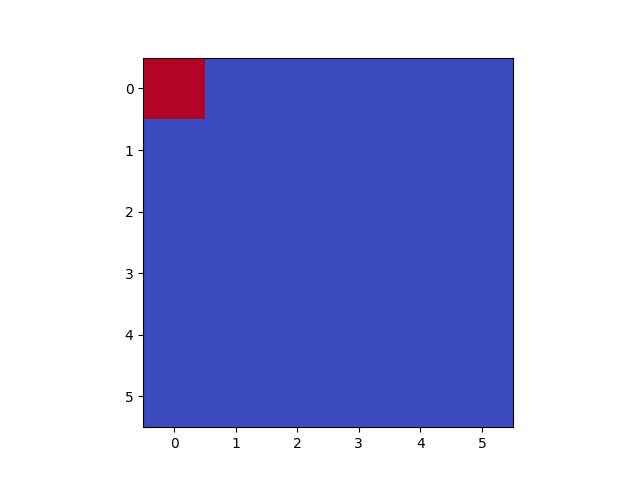
\includegraphics[width=3cm]{../plots/beta_ols_visualize.png} }}%
	\subfloat[Ridge self]{{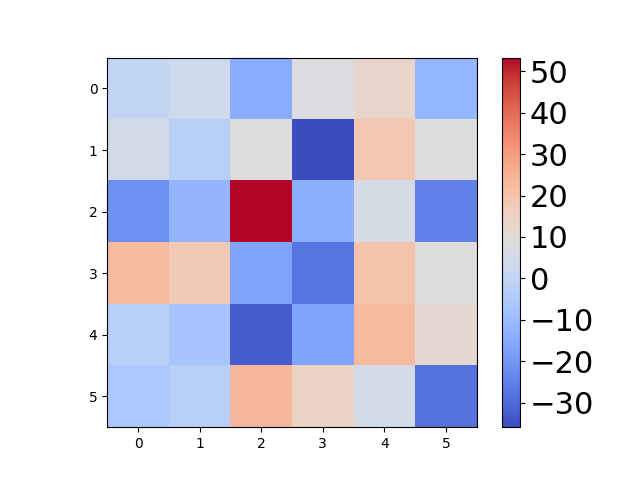
\includegraphics[width=3cm]{../plots/beta_ridge_visualize.png} }}%
	\subfloat[Lasso self]{{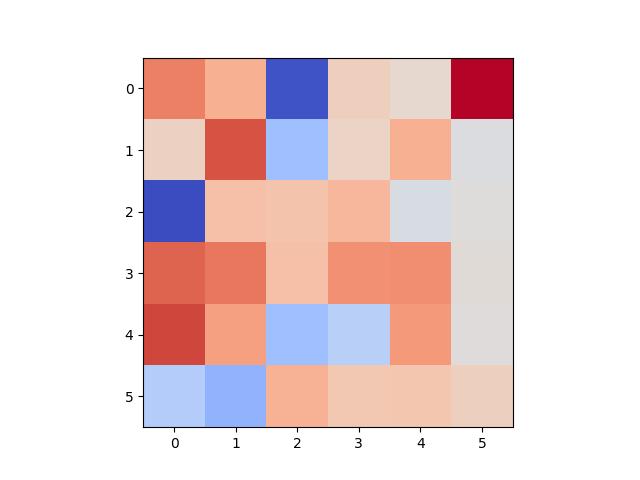
\includegraphics[width=3cm]{../plots/beta_lasso_visualize.png} }}%
	\subfloat[Ridge2 self]{{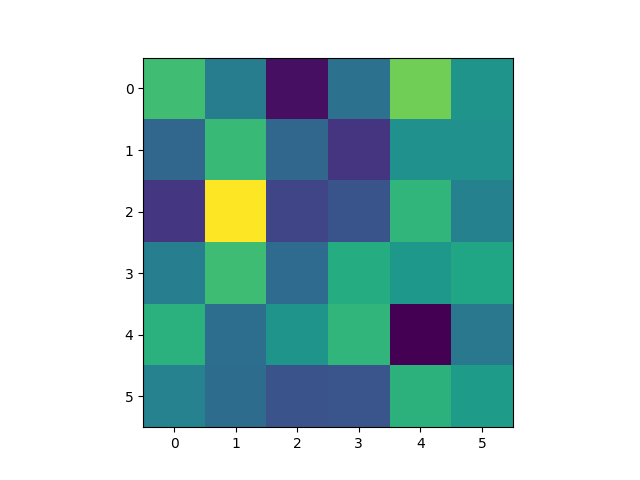
\includegraphics[width=3cm]{../plots/beta_ridge2_visualize.png} }}\\
	
	\subfloat[OLS scikit]{{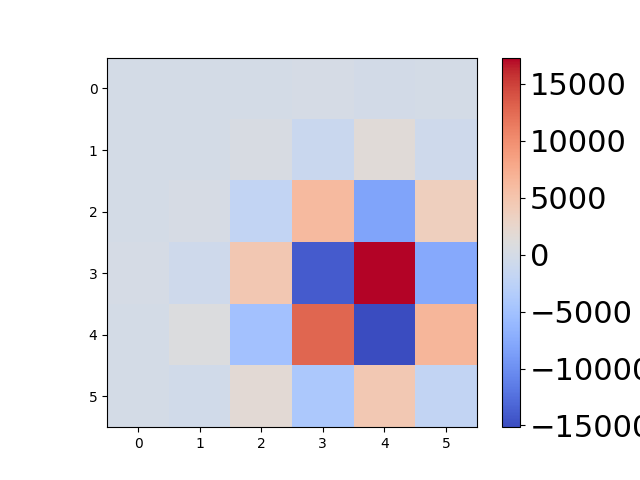
\includegraphics[width=3cm]{../plots/beta_ols_test_visualize.png} }}%
	\subfloat[Ridge scikit]{{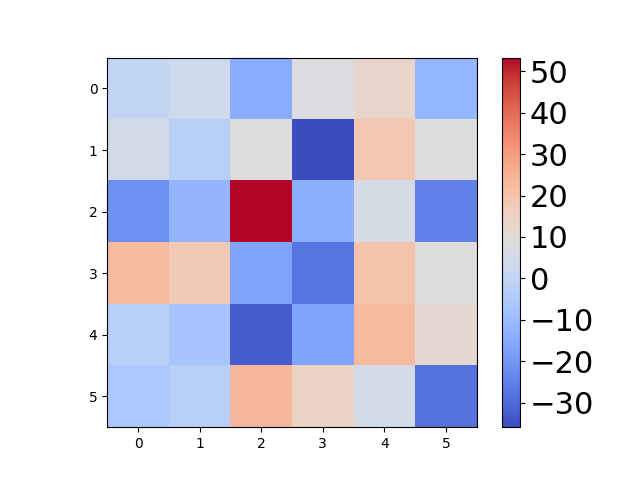
\includegraphics[width=3cm]{../plots/beta_ridge_test_visualize.png} }}%
	\subfloat[Lasso scikit]{{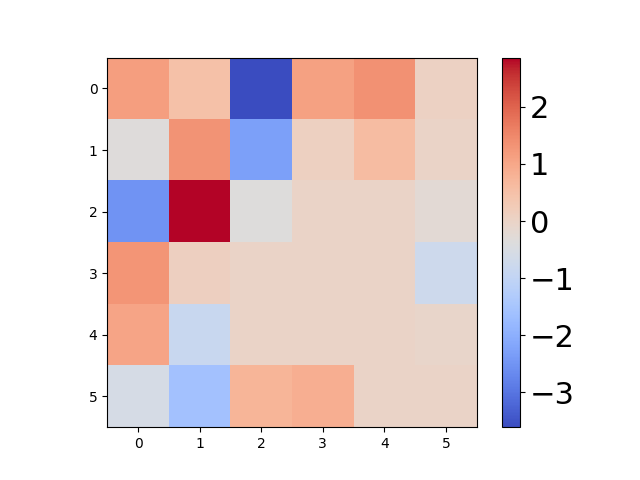
\includegraphics[width=3cm]{../plots/beta_lasso_test_visualize.png} }}%
	\subfloat[Ridge scikit]{{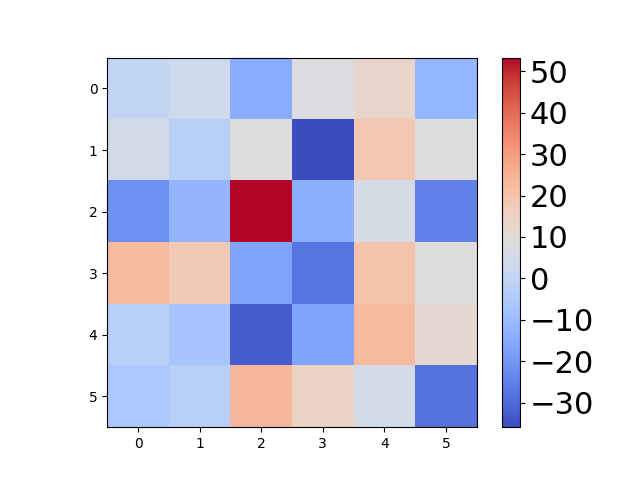
\includegraphics[width=3cm]{../plots/beta_ridge_test_visualize.png} }}
	
	\caption{Beta values visualized for different methods. The upper images are gotten from the self-built functions, where the last one is Ridge found by minimizing beta using gradient descent. The lower images are the benchmarks which are produced by Scikit learn.}%
	\label{fig:beta_plots}%
\end{figure}

Furthermore, the confidence intervals are given in table \eqref{tab:CI_franke} for all betas and all methods.

\begin{table} [H]
	\caption{Write table text here.  \vspace{2mm}}
	\begin{tabularx}{\textwidth}{l|XXXX} \hline\hline
		\label{tab:CI_franke}
		&\textbf{OLS}&\textbf{Ridge}&\textbf{Lasso}&\textbf{Ridge2}\\ \hline \\
		$\beta_1$ & 0.07853 & 0.86104 & 0.05386 & 1.7483\\
		$\beta_2$ & 0.07853 & 0.86104 & 0.05386 & 1.7483\\
		$\beta_3$ & 0.07853 & 0.86104 & 0.05386 & 1.7483\\
		$\beta_4$ & 0.07853 & 0.86104 & 0.05386 & 1.7483\\
		$\beta_5$ & 0.07853 & 0.86104 & 0.05386 & 1.7483\\
		$\beta_6$ & 0.07853 & 0.86104 & 0.05386 & 1.7483\\
		$\beta_7$ & 0.07853 & 0.86104 & 0.05386 & 1.7483\\
		$\beta_8$ & 0.07853 & 0.86104 & 0.05386 & 1.7483\\
		$\beta_9$ & 0.07853 & 0.86104 & 0.05386 & 1.7483\\
		$\beta_{10}$ & 0.07853 & 0.86104 & 0.05386 & 1.7483\\
		$\beta_{11}$ & 0.07853 & 0.86104 & 0.05386 & 1.7483\\
		$\beta_{12}$ & 0.07853 & 0.86104 & 0.05386 & 1.7483\\
		$\beta_{13}$ & 0.07853 & 0.86104 & 0.05386 & 1.7483\\
		$\beta_{14}$ & 0.07853 & 0.86104 & 0.05386 & 1.7483\\
		$\beta_{15}$ & 0.07853 & 0.86104 & 0.05386 & 1.7483\\
		$\beta_{16}$ & 0.07853 & 0.86104 & 0.05386 & 1.7483\\
		$\beta_{17}$ & 0.07853 & 0.86104 & 0.05386 & 1.7483\\
		$\beta_{18}$ & 0.07853 & 0.86104 & 0.05386 & 1.7483\\
		$\beta_{19}$ & 0.07853 & 0.86104 & 0.05386 & 1.7483\\
		$\beta_{20}$ & 0.07853 & 0.86104 & 0.05386 & 1.7483\\
		$\beta_{21}$ & 0.07853 & 0.86104 & 0.05386 & 1.7483\\
		$\beta_{22}$ & 0.07853 & 0.86104 & 0.05386 & 1.7483\\
		$\beta_{23}$ & 0.07853 & 0.86104 & 0.05386 & 1.7483\\
		$\beta_{24}$ & 0.07853 & 0.86104 & 0.05386 & 1.7483\\
		$\beta_{25}$ & 0.07853 & 0.86104 & 0.05386 & 1.7483\\
		$\beta_{26}$ & 0.07853 & 0.86104 & 0.05386 & 1.7483\\
		$\beta_{27}$ & 0.07853 & 0.86104 & 0.05386 & 1.7483\\
		$\beta_{28}$ & 0.07853 & 0.86104 & 0.05386 & 1.7483\\
		$\beta_{29}$ & 0.07853 & 0.86104 & 0.05386 & 1.7483\\
		$\beta_{30}$ & 0.07853 & 0.86104 & 0.05386 & 1.7483\\
		$\beta_{31}$ & 0.07853 & 0.86104 & 0.05386 & 1.7483\\
		$\beta_{32}$ & 0.07853 & 0.86104 & 0.05386 & 1.7483\\
		$\beta_{33}$ & 0.07853 & 0.86104 & 0.05386 & 1.7483\\
		$\beta_{34}$ & 0.07853 & 0.86104 & 0.05386 & 1.7483\\
		$\beta_{35}$ & 0.07853 & 0.86104 & 0.05386 & 1.7483\\
		$\beta_{36}$ & 0.07853 & 0.86104 & 0.05386 & 1.7483\\ \hline
	\end{tabularx}
\end{table}

\subsection{Real data}
Below one can find the results of the regression on Franke function. All results in this section was obtained from the same data set, with an estimated variance of ...

\subsubsection{Visualization of graphes}
In figure \eqref{fig:franke} one can find a 3D visualization of the Franke function, for easier comparison with the fitted graphs presented in figure \eqref{fig:franke_plots}. The data sets were composed drawing random $x$'s and $y$'s in the interval $x,y\in[0,1]$ from a uniform distribution, and the corresponding $z$-values where obtained from the Franke function. Further, we added noise produced by $\mathcal{N}(0, \sigma^2=0.1)$ and compared with the undisturbed data set. For Lasso and Ridge, we used a penalty $\lambda=1e-15$, and for Lasso we also used gradient descent for minimization. On that occasion, the learning rate was set to $\eta=0.001$ with niter$=1000000$ as the number of iterations. 


\newgeometry{left=2cm,right=2cm,top=1cm}
\begin{figure} [H]%
	\centering
	\subfloat[OLS without noise]{{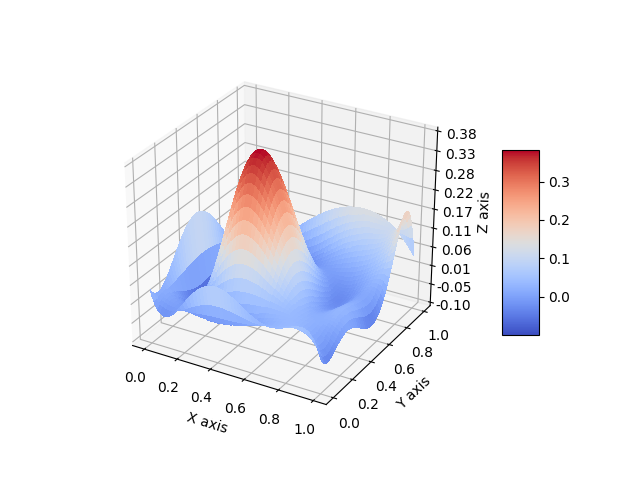
\includegraphics[width=9cm]{../plots/OLS_terrain.png} }}%
	\subfloat[OLS with noise]{{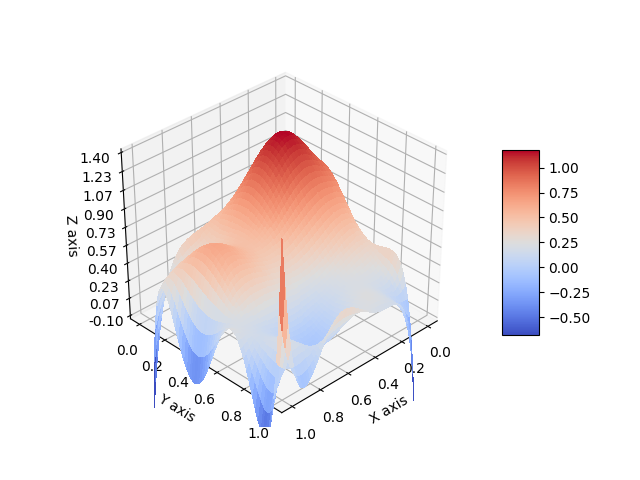
\includegraphics[width=9cm]{../plots/OLS_noise.png} }}\\
	
	\subfloat[Ridge without noise]{{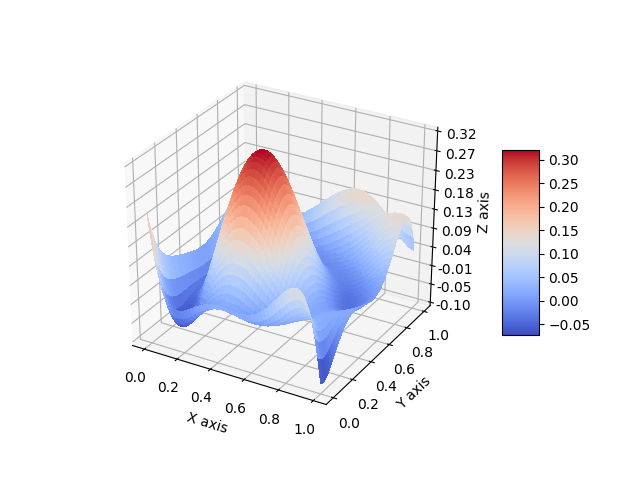
\includegraphics[width=9cm]{../plots/Ridge_terrain.png} }}%
	\subfloat[Ridge with noise]{{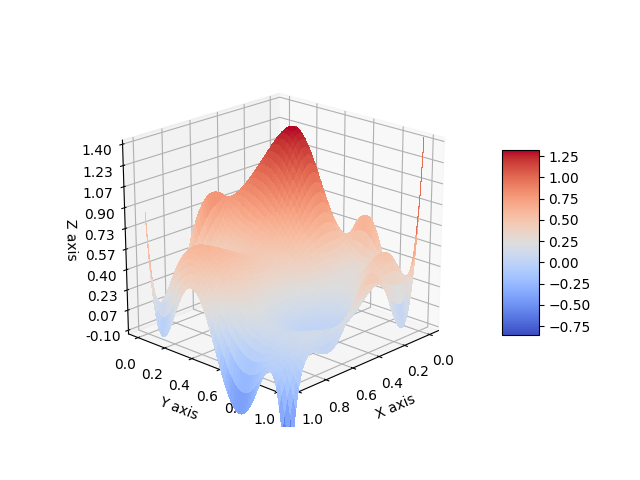
\includegraphics[width=9cm]{../plots/Ridge_noise.png} }}\\
	
	\subfloat[Lasso without noise]{{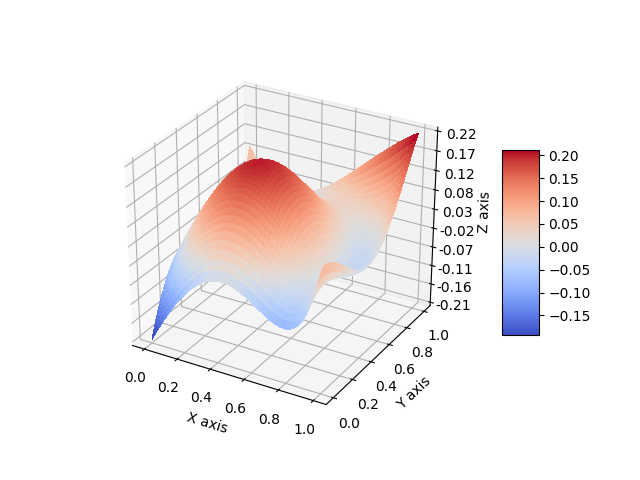
\includegraphics[width=9cm]{../plots/Lasso_terrain.png} }}%
	\subfloat[Lasso with noise]{{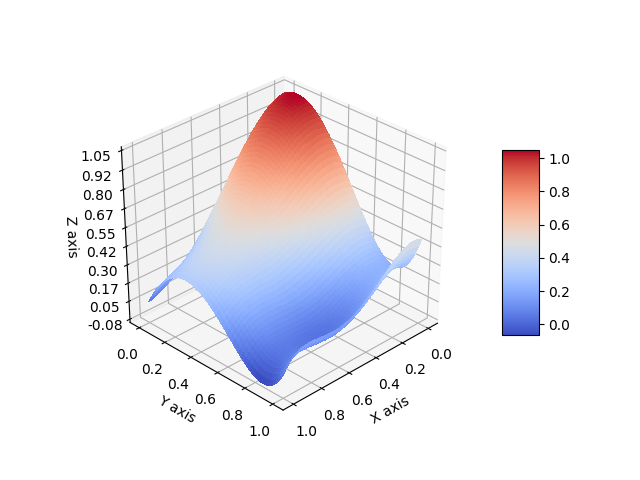
\includegraphics[width=9cm]{../plots/Lasso_noise.png} }}
	\caption{Fitted polynomial by OLS, Ridge and Lasso with and without noise. For Ridge and Lasso, we used a low penalty of $\lambda=1e-15$. Lasso was performed with $\eta=1e-3$ and 1e6 iterations. The noise was sampled from a normal distribution with $\sigma=0.1$.}%
	\label{fig:franke_plots}%
\end{figure}
\restoregeometry


\subsubsection{Error}
To be able to determine which method is best, we need to analyze the error. In table \eqref{tab:franke_error}, the MSE and R$^2$-score are given for OLS, Ridge, Lasso and Ridge with gradient descent. 

\begin{table} [H]
	\caption{Mean Square Error and R$^2$-score presented for OLS, Ridge, Lasso and Ridge + gradient descent.  \vspace{2mm}}
	\begin{tabularx}{\textwidth}{l|XX|XX} \hline\hline
		\label{tab:franke_error}
		& \multicolumn{2}{c}{\textbf{MSE}}&\multicolumn{2}{c}{\textbf{R2}}\\ \hline
		&self&scikit&self&scikit\\ \hline \\
		OLS & 0.07853 & 0.86104 & 0.05386 & 1.7483\\
		Ridge & 0.07852 & 0.86410 & 0.05406 & 1.6904 \\
		Lasso & 0.07704 & 0.86231 & 0.07187 & 1.6492 \\
		RidgeGD & 0.07523 & 0.91850 & 0.09362 & 1.3217 \\ \hline
	\end{tabularx}
\end{table}


\subsubsection{Confidence interval}
It can also be interesting to see how the coefficients actually differ between the self-built functions and the Scikit Learn function. In figure \eqref{fig:beta_plots}, the beta values are visualized such that large numbers got strong color, negative numbers are blue and positive numbers are red. The methods OLS, Ridge, Lasso and Ridge produced using gradient descent are presented. 



Furthermore, the confidence intervals are given in table \eqref{tab:CI_franke} for all betas and all methods.

\begin{table} [H]
	\caption{Write table text here.  \vspace{2mm}}
	\begin{tabularx}{\textwidth}{l|XXXX} \hline\hline
		\label{tab:CI_franke}
		&\textbf{OLS}&\textbf{Ridge}&\textbf{Lasso}&\textbf{Ridge2}\\ \hline \\
		$\beta_1$ & 0.07853 & 0.86104 & 0.05386 & 1.7483\\
		$\beta_2$ & 0.07853 & 0.86104 & 0.05386 & 1.7483\\
		$\beta_3$ & 0.07853 & 0.86104 & 0.05386 & 1.7483\\
		$\beta_4$ & 0.07853 & 0.86104 & 0.05386 & 1.7483\\
		$\beta_5$ & 0.07853 & 0.86104 & 0.05386 & 1.7483\\
		$\beta_6$ & 0.07853 & 0.86104 & 0.05386 & 1.7483\\
		$\beta_7$ & 0.07853 & 0.86104 & 0.05386 & 1.7483\\
		$\beta_8$ & 0.07853 & 0.86104 & 0.05386 & 1.7483\\
		$\beta_9$ & 0.07853 & 0.86104 & 0.05386 & 1.7483\\
		$\beta_{10}$ & 0.07853 & 0.86104 & 0.05386 & 1.7483\\
		$\beta_{11}$ & 0.07853 & 0.86104 & 0.05386 & 1.7483\\
		$\beta_{12}$ & 0.07853 & 0.86104 & 0.05386 & 1.7483\\
		$\beta_{13}$ & 0.07853 & 0.86104 & 0.05386 & 1.7483\\
		$\beta_{14}$ & 0.07853 & 0.86104 & 0.05386 & 1.7483\\
		$\beta_{15}$ & 0.07853 & 0.86104 & 0.05386 & 1.7483\\
		$\beta_{16}$ & 0.07853 & 0.86104 & 0.05386 & 1.7483\\
		$\beta_{17}$ & 0.07853 & 0.86104 & 0.05386 & 1.7483\\
		$\beta_{18}$ & 0.07853 & 0.86104 & 0.05386 & 1.7483\\
		$\beta_{19}$ & 0.07853 & 0.86104 & 0.05386 & 1.7483\\
		$\beta_{20}$ & 0.07853 & 0.86104 & 0.05386 & 1.7483\\
		$\beta_{21}$ & 0.07853 & 0.86104 & 0.05386 & 1.7483\\
		$\beta_{22}$ & 0.07853 & 0.86104 & 0.05386 & 1.7483\\
		$\beta_{23}$ & 0.07853 & 0.86104 & 0.05386 & 1.7483\\
		$\beta_{24}$ & 0.07853 & 0.86104 & 0.05386 & 1.7483\\
		$\beta_{25}$ & 0.07853 & 0.86104 & 0.05386 & 1.7483\\
		$\beta_{26}$ & 0.07853 & 0.86104 & 0.05386 & 1.7483\\
		$\beta_{27}$ & 0.07853 & 0.86104 & 0.05386 & 1.7483\\
		$\beta_{28}$ & 0.07853 & 0.86104 & 0.05386 & 1.7483\\
		$\beta_{29}$ & 0.07853 & 0.86104 & 0.05386 & 1.7483\\
		$\beta_{30}$ & 0.07853 & 0.86104 & 0.05386 & 1.7483\\
		$\beta_{31}$ & 0.07853 & 0.86104 & 0.05386 & 1.7483\\
		$\beta_{32}$ & 0.07853 & 0.86104 & 0.05386 & 1.7483\\
		$\beta_{33}$ & 0.07853 & 0.86104 & 0.05386 & 1.7483\\
		$\beta_{34}$ & 0.07853 & 0.86104 & 0.05386 & 1.7483\\
		$\beta_{35}$ & 0.07853 & 0.86104 & 0.05386 & 1.7483\\
		$\beta_{36}$ & 0.07853 & 0.86104 & 0.05386 & 1.7483\\ \hline
	\end{tabularx}
\end{table}